\subsection{The Conjugate gradient method}

\subsubsection{Motivation}

\notesonly{
We have seen how line search allows us to reach the minimum along the direction of the gradient $\vec g_t$ computed at time step $t$. It achieves this by manipulating the magnitude of the step we take towards a lower cost.
Looking at what happens over multiple time steps we observe the following movements on the surface of the cost function:
}
\begin{frame}{Limitations of line search}

\begin{center}
	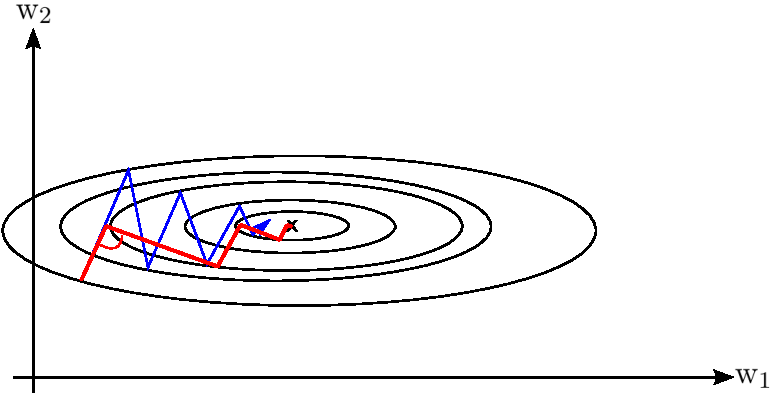
\includegraphics[width=0.6\textwidth]{img/section1_fig23_clean_ls}
	\captionof{figure}{Weight updates by following line search 
	%(\textcolor{red}{red}).}
	(red).}
\end{center}

\mode<presentation>{
	\only<2>{
		\begin{center}
			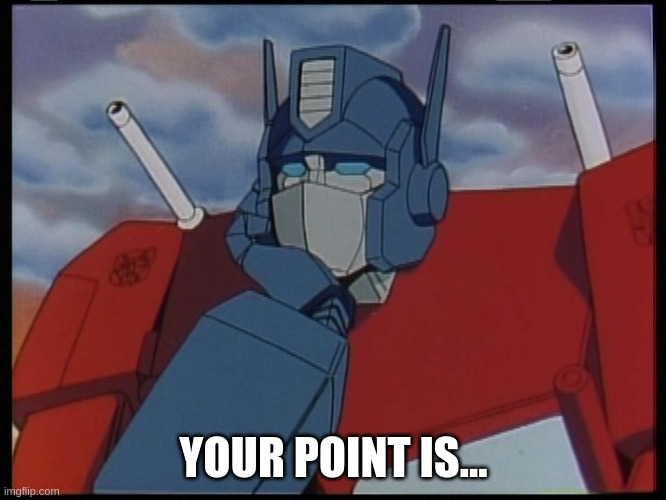
\includegraphics[width=0.3\textwidth]{img/meme_point}
		\end{center}
	}
	\only<3>{
		\begin{center}
			
\includegraphics[width=0.3\textwidth]{img/meme_deeper}
		\end{center}
	}
	\only<4>{
		\begin{center}
			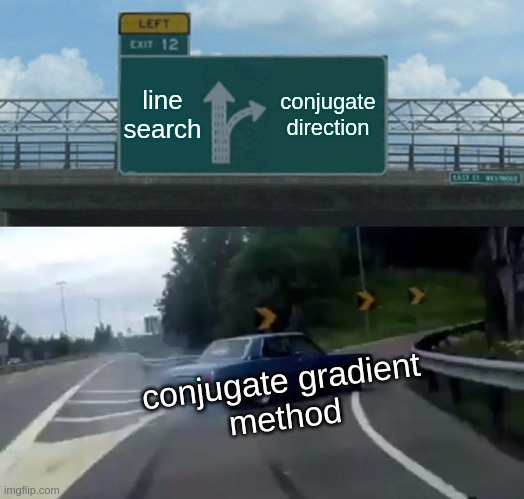
\includegraphics[width=0.3\textwidth]{img/meme_direction}
		\end{center}
	}
}

\end{frame}

\begin{frame}{Limitations of line search}
		\begin{center}
			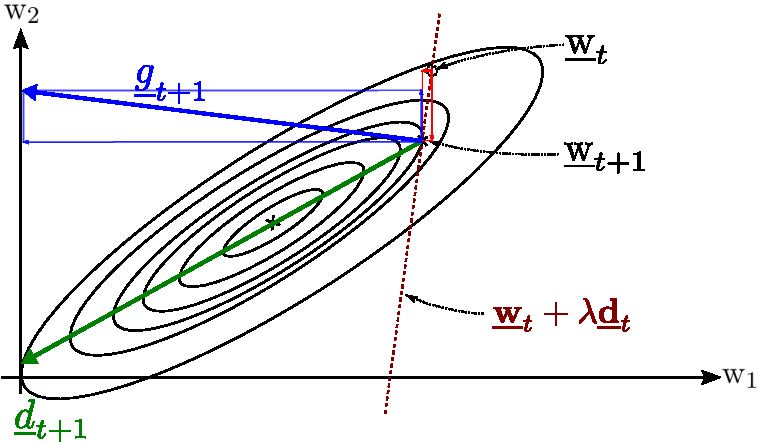
\includegraphics[width=0.8\textwidth]{img/conjugate_direction_c}
			\notesonly{
			\captionof{figure}{The conjugate direction avoids undoing progress made in the previous step.}
			}
		\end{center}
\end{frame}

\begin{frame}\frametitle{Conjugate gradient method}
\mode<article>{
\underline{Conjugate gradient method}:

}

		\begin{eqnarray}
			\vec{w}_{t+1}
			%& = & \mathrm{w}_{ij}(t) 
			%+ \Delta \mathrm{w}_{ij}(t)  \\ 
			& =&  \vec{w}_t + \eta_t \, \vec{d}_{t-1}
		\end{eqnarray}

Don't undo progress of previous search directions $\vec d_{t}$, $\vec d_{t-1}$.

In other words:

The component of the gradient parallel to the old direction $\vec d_{t}$ should
remain zero along the new direction $\vec d_{t+1}$

\pause
	
	\begin{block}{$ $}
		\textbf{Initialization:} $\vec{w},\quad \vec{d} = - \vec{g}$\\
		\vspace{3mm}

		\While{stopping criterion not fulfilled}{
			\vspace{1mm}
			Minimize $E^T$ along $\vec{d}$ using line-search 
				\quad $\rightarrow$ new $\vec{w}$ \\[1mm]
			Calculate the new conjugate direction 
				\quad $\;\,\rightarrow$ new $\vec{d}$
			\vspace{1mm}
		}
	\end{block}

\end{frame}

% -----------------------------------------------------------------------------
\begin{frame}\frametitle{Adaptive momentum: the Polak-Ribiere rule}
	\begin{equation}\tag{conjugate direction}
		\vec{d}_{t+1} = - 
		\overbrace{\frac{\partial E^T}{\partial \vec{w}}
			\bigg|_{\vec{w}_{t+1}}}^{\vec{g}_{t+1}} + \beta_t \, \vec{d}_t
	\end{equation}%\\[5mm]
	\begin{equation}\tag{``smart momentum''}
		\beta_t = \underbrace{ \frac{\vec{g}_{t+1}^\top
			\big( \vec{g}_{t+1} - \vec{g}_t \big)}{
			\vec{g}_t^\top \vec{g}_t} }_{
				\text{Polak-Ribiere rule}}
	\end{equation}
	OR
			  \begin{equation} %\tag{Fletcher-Reeves form}
		  		\beta_t = \underbrace{-\frac{\vec{g}_{t+1}^\top\vec{g}_{t+1}}%
		  		{\vec{g}_t^\top\vec{g}_t}}_{\text{Fletcher-Reeves}}.
		  \end{equation} 
	%\iitem{determine learning rate $\eta_t$ via line search}
\end{frame}

% -----------------------------------------------------------------------------
\begin{frame}\frametitle{Conjugate gradient descent algorithm}
\slidesonly{
	\begin{block}{$ $}
		\textbf{Initialization:} $\vec{w},\quad \vec{d} = - \vec{g}$\\
		\vspace{3mm}

		\While{stopping criterion not fulfilled}{
			\vspace{1mm}
			Minimize $E^T$ along $\vec{d}$ using line-search 
				\quad $\rightarrow$ new $\vec{w}$ \\[1mm]
			Calculate the new conjugate direction 
				\quad $\;\,\rightarrow$ new $\vec{d}$
			\vspace{1mm}
		}
	\end{block}
	}
	\iitem{Subsequent search directions lose conjugacy 
		\iitem{search direction should be reset to the 	steepest \\ 
			descent direction at least every $N$ iterations (in practice apply heuristic, e.g. reset every 5 steps)}
	}
\end{frame}

\slidesonly{
\begin{frame} \frametitle{Comparison}
\placeimage{0.5}{2.5}{img/section1_fig23_clean}{width=6cm}
\placeimage{8}{2.5}{img/section1_fig24_clean}{width=6cm}
\placeimage{0.5}{8.5}{img/section1_fig23_clean_ls}{width=6cm}
\placeimage{8}{8.5}{img/section1_fig23_clean_conj}{width=6cm}
\end{frame}
}
